% Figura — Curva conceitual de eficiência do pipeline (Cap. 5)
\begin{figure}[!htb]
\centering
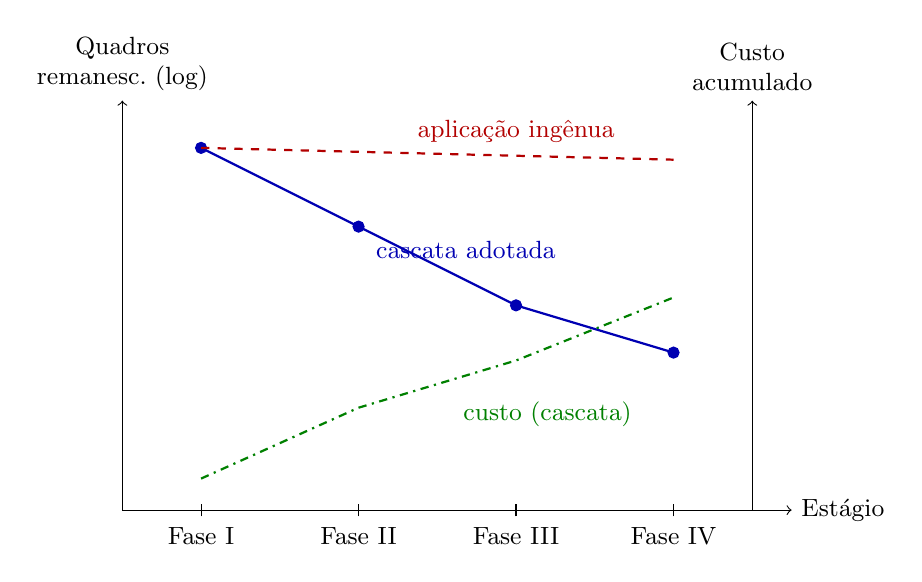
\begin{tikzpicture}[font=\small]
\begin{scope}
  % eixos
  \draw[->] (0,0) -- (8.5,0) node[right]{Estágio};
  \draw[->] (0,0) -- (0,5.2) node[above, align=center]{Quadros\\remanesc.\ (log)};
  \draw[->] (8.0,0) -- (8.0,5.2) node[above, align=center]{Custo\\acumulado};

  % marcas x
  \foreach \x/\v in {1/Fase I, 3/Fase II, 5/Fase III, 7/Fase IV} {
    \draw (\x,-0.08) -- (\x,0.08);
    \node[below] at (\x,-0.1) {\v};
  }

  % cascata adotada (queda monotônica)
  \draw[thick, blue!70!black]
    plot coordinates {(1,4.6) (3,3.6) (5,2.6) (7,2.0)};
  \foreach \p in {(1,4.6),(3,3.6),(5,2.6),(7,2.0)} \filldraw[blue!70!black] \p circle (2pt);
  \node[blue!70!black, anchor=west] at (3.1,3.3) {cascata adotada};

  % aplicação ingênua (reta horizontal)
  \draw[thick, red!70!black, dashed]
    plot coordinates {(1,4.6) (3,4.55) (5,4.5) (7,4.45)};
  \node[red!70!black, anchor=south] at (5.0,4.55) {aplicação ingênua};

  % custo acumulado (cascata, crescente moderado)
  \draw[thick, green!50!black, dash dot]
    plot coordinates {(1,0.4) (3,1.3) (5,1.9) (7,2.7)};
  \node[green!50!black, anchor=north] at (5.4,1.50) {custo (cascata)};

\end{scope}
\end{tikzpicture}
\caption{Curva conceitual de eficiência do pipeline em cascata em comparação à aplicação ingênua das fases sobre todos os quadros: queda monotônica do volume (eixo $y$ esquerdo, escala logarítmica) contrastada com o custo computacional acumulado (eixo $y$ direito). \obsfic{traços ilustrativos; substituir pelas curvas empíricas após execução.}}
\label{fig:res-eficiencia}
\end{figure}
